\documentclass{standalone}
\usepackage{tikz}
\usepackage{pgfplots}
\usepgfplotslibrary{colormaps}
\pgfplotsset{colormap/copper2}

\begin{document}
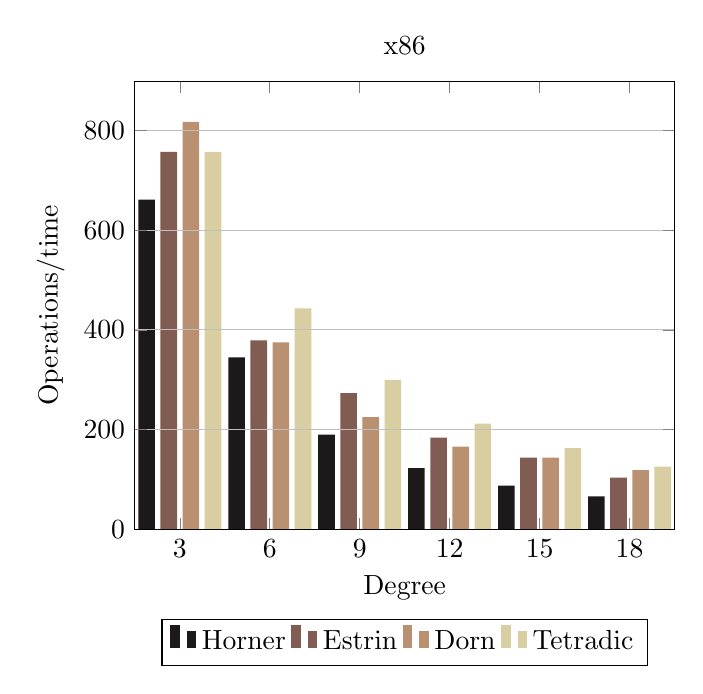
\begin{tikzpicture}

  \begin{axis}[
      ybar,
      axis on top,
      bar width=6pt,
      ymin=0,
      ymajorgrids,
      tick align=inside,
      xtick=data,
      symbolic x coords={3, 6, 9, 12, 15, 18},
      legend style={at={(0.5,-0.2)},anchor=north,legend columns=-1},
      title={x86},
      xlabel={Degree},
      ylabel={Operations/time},
      colormap name=copper2
    ]
    % Horner
    \addplot [color of colormap={100},draw=none,fill=.] coordinates {
      (3, 661)
      (6, 345)
      (9, 190)
      (12, 123)
      (15, 88)
      (18, 66)
    };
    \addlegendentry{Horner};
    % Estrin
    \addplot [color of colormap={400},draw=none,fill=.] coordinates {
      (3, 757)
      (6, 379)
      (9, 273)
      (12, 184)
      (15, 144)
      (18, 104)
    };
    \addlegendentry{Estrin};
    % Dorn
    \addplot [color of colormap={600},draw=none,fill=.] coordinates {
      (3, 817)
      (6, 375)
      (9, 225)
      (12, 166)
      (15, 144)
      (18, 119)
    };
    \addlegendentry{Dorn};
    % Tetradic
    \addplot [color of colormap={800},draw=none,fill=.] coordinates {
      (3, 757)
      (6, 443)
      (9, 300)
      (12, 212)
      (15, 163)
      (18, 126)
    };
    \addlegendentry{Tetradic};
  \end{axis}

\end{tikzpicture}
\end{document}
